

\section{Results and Analysis}
\label{sec-results}

%In this section, we report the results of our empirical evaluations to answer the three research questions.
 
This section reports the data we collected to empirically address the three research questions, their interpretations, and our results.

%\vspace{-0.4cm} 
\subsection{RQ1: Accuracy}


Table~\ref{tab:tab-results} summarizes the results of our
experiments for evaluating the accuracy of \@approach in
detecting compatibility issues compared to the other
state-of-the-art and state-of-the-practice techniques.  For
each app under analysis, we report the number of true (\tp)
and false (\fp) positives and false negatives (\fn)
according to the three categories of compatibility issues:

\textbf{API Invocation Compatibility Issues (API).}
\@approach succeeds in detecting all 8 known API
compatibility issues in \textsc{CiD}-Bench suite, and 33 API
compatibility issues out of 36 in \textsc{Cider}-Bench
suite.  It also correctly ignores 32 cases in \texttt{FOSS
Browser}, \texttt{Padland}, \texttt{DuckDuckGo},
\texttt{SurvivalManual} and \texttt{Uber~ride} apps, where
there are no API compatibility issues yet wrongly reported
by \textsc{CiD}. The only missed issues are the ones that
occur in the \texttt{MaterialFBook} app's anonymous classes,
not handled by our model extractor, discussed in more detail
in Section~\ref{sec-discussion}.  {\sc Cid} detects fewer
(26 out of 44) API invocation compatibility issues, and it has a high rate of
false positives, the majority of which arise because
\textsc{CiD}'s analysis is not context-sensitive and does
not track guard conditions across function calls.
\textsc{Lint} does even worse and only identified one of the
verified mismatches.  According to the results,
\textsc{Cider} is unable to examine Android apps for API
invocation compatibility issues. The results show that
\@approach outperforms the other three techniques in terms
of both precision and recall.


\textbf{API Callback Compatibility Issues (APC).} \@approach
successfully detects 40 callback compatibility issues out of
42 in the objects of analysis, with no false positives.
{\sc Cider} misses most of the issues identified by
\@approach mainly because it only considers the classes that
were manually modeled, i.e., {\sf Activity}, {\sf Fragment},
{\sf Service}, and {\sf WebView}. Whereas, \@approach
automatically identifies potential callback mismatches
across all classes in the Android API.  As expected,
\textsc{CiD} is unable to examine Android apps for callback
compatibility issues. \textsc{Lint} not only identifies none
of the verified mismatches, but also has a high rate of
false warnings. Overall, the results show that \@approach
outperforms the other three techniques in terms of both
precision and recall.


\textbf{Permission-induced Compatibility Issues (PRM).}
According to the experimental results, %shown in Table~\ref{tab:tab-results}, 
\@approach detects two cases of permission-induced compatibility issues in
\textit{FOSS Browser}~\cite{fossbrowser} and
\textit{Kolab notes}~\cite{kolab} apps; these two apps
request dangerous permissions and target an API level
higher than 23, yet they do not follow the new runtime
permission checking. Note that the other mismatch
detection techniques do not detect any of the runtime
permission compatibility issues.  Next, we evaluate
whether \@approach is sufficiently robust to handle
large real-world apps.


\subsection{RQ2: Real-World Applicability}

To evaluate the implications of our tool in practice, we applied \@approach to real-world apps collected from a variety of repositories (cf. Section~\ref{sec-eval}).
%When applied to real-world apps, 
\@approach detected 68,268 potential API invocation mismatches, with 41.19\% of the
apps harboring at least one potential mismatch. It also
identified 2,115 potential API callback mismatches occurring
in 20.05\% of the apps under analysis.  To perform the
permission-induced mismatch analysis, we divided the apps
into two groups based on the target SDK version: (i) 1,815
apps target Android API levels greater than or equal to 23
and (ii) 1,756 apps target Android API levels below 23. We
identified a total of 1,430 apps across both groups with at
least one permissions-induced compatibility issue. 224 apps
(12.34\%) in group (i) attempt to use dangerous permissions
without implementing the runtime permissions request system,
and 1,206 apps (68.68\%) in group (ii) are vulnerable to
permissions revocation mismatches (cf.
Section~\ref{sec-background:prm}).

%\commentty{added text below.}
Since manually examining all 3,691 real-world apps 
prohibitively expensive, we sampled 60 apps where 
incompatibilities were detected and calculated 
the precision scores. We do not consider
recall because the ground-truth incompatibilities
are unknown. Among all 60 incompatibility issues,
the precision scores for API invocation, callback, and permission
incompatibilities are 85\%, 100\%, and 100\%, respectively. 
The results are consistent with the ones obtained from the benchmark programs (cf. Table~\ref{tab:tab-results}). 

%Because the apps in group (i) are more recent, they are
%also representative of apps that are currently used on
%devices.  Therefore, we further investigate the usage
%of dangerous permissions among the apps in this group.
%After studying the apps, we realized that these apps
%only use 10 out of 26 dangerous
%permissions~\cite{dangerousAPI}. Within the group, 127
%apps, mostly targeting API level 23, requested these 10
%permissions. The permission WRITE\_EXTERNAL\_STORAGE is
%the most requested by applications (110 times),
%followed by READ\_EXTERNAL\_STORAGE (47 times) and
%READ\_PHONE\_STATE (31 times). Some dangerous
%permissions such as READ\_CALENDAR, WRITE\_CALENDAR and
%READ\_CONTACTS were not requested at all.
 
We then investigated the \@approach's results to
appraise its utility in practice. In the following, we
report some of our findings. To avoid revealing previously
unknown compatibility issues, we only disclose a subset of
those that we have had the opportunity to bring to the app
developers' attention.

%\commentty{where are the results below from? I assume they are not from the 68,268 apps? We should clarify}


%API invocation -> org.sufficientlysecure.localcalendar_9:

\textbf{API invocation mismatch.} In the \textsf{Offline
Calendar} app~\cite{offlinecalendar}, the invocation of the
\textsf{getFragmentManager()} API method in
\textsf{PreferencesActivity.onCreate} causes an API
invocation mismatch.  The \textsf{getFragmentManager()}
method was added to the \textsf{Activity} class in API level
11. Yet, \textsf{Offline Calendar} sets its
\textsf{minSdkVersion} to API level 8. Therefore, as soon as
the \textsf{PreferencesActivity} is activated, the
\textsf{Offline Calendar} app will crash if running on API
levels 8 to 11. The mismatch could be resolved by wrapping
the call to \textsf{getFragmentManager()} in a guard
condition to only execute it if the device's API level is
equal or greater than 11, or by setting the
\textsf{minSdkVersion} to 11.
%API callback -> be.digitalia.fosdem_1500150:

\textbf{API callback mismatch.} FOSDEM~\cite{fosdem} is a
conference companion app.  It exhibits an API callback
mismatch in its \textsf{ForegroundLinearLayout} class, which
overrides the \textsf{View.drawableHotspotChanged} callback
method, introduced in API level 21. However, its
\textsf{minSdkVersion} is set to API level 15, which would
not support the aforementioned callback method, and in turn
may not properly propagate the new hotspot location to the
\textsf{Drawable} stored as a member of the layout class.
This could lead to crashes or other instability in the app
interface. Setting the \textsf{minSdkVersion} to 21 would
resolve the mismatch.



%permission request mismatch -> org.kore.kolabnotes.android_98:

\textbf{Permission request mismatch.} \textsf{Kolab
Notes}~\cite{kolab} is a note-taking app that can
synchronize notes with other apps.  It exhibits a permission
request mismatch. The app targets API 26 and uses the
\textsf{WRITE}$\_$\textsf{EXTERNAL}$\_$\textsf{STORAGE}
permission, but does not implement the necessary methods to
request the permission at runtime. If the permission is not
already granted when the user attempts to save or load data
to/from an SD card, the action will fail. To resolve the
mismatch, the developers should update the app to implement
the new runtime permissions request system, particularly the
\textsf{onRequestPermissionsResult} callback.

\textbf{Permission revocation mismatch.}
%-> org.adaway_3.0.2:
\textsf{AdAway}~\cite{adaway} is an ad blocking app that
suffers from a permission revocation mismatch. The app
targets API level 22 and uses the
\textsf{WRITE}$\_$\textsf{EXTERNAL}$\_$\textsf{STORAGE}
permission, which could be revoked by the user when
installed on a device running API 23 or greater. If the user
revokes the permission and tries to export a file, the app
will crash. The developers could resolve the issue by
updating the app to use runtime permissions and setting the
\textsf{minSdkVersion} to 23.



%\begin{sidewaystable}
%\scriptsize
%\centering
%\begin{threeparttable}[c]
%\begin{table}[b!]
\begin{table}%{r}{0.4\linewidth}
\centering
%\begin{tiny}
%\begin{small}
%\begin{footnotesize}
\begin{scriptsize}
%\vspace{-0.8cm}
\caption {\label{tab:tab-timing-results} Experiments performance statistics in seconds.}
\vspace{-0.1cm}
\begin{tabular}{c|l|r|r|r}
\hline
\hline
\rule{0pt}{3ex}
%&     & \multicolumn{1}{|c}{\sc GAINDroid} & \multicolumn{4}{|c}{\sc CiD\tnote{1}} & \multicolumn{3}{|@{\hspace{0.5em}}c@{\hspace{0.5em}}}{\sc Cider\tnote{2}} & \multicolumn{4}{|c}{\sc Lint} \\
& App      & {\sc SAINT}  & {\sc CiD}     & {\sc Lint} \\
&       & {\sc Droid}  &       &   \\
\hline
\hline
\rule{0pt}{3ex}
\parbox[t]{5mm}{\multirow{12}{*}{\rotatebox[origin=c]{90}{\textsc{Cider}-Bench}}}
& AFWall+         & 8.2  & -- %$\infty$
& 41.3 \\
& DuckDuckGo      & 7.7  & 60.3     & 35.1 \\
& FOSS Browser    & 3.6  & 17.2     & 30.3 \\
& Kolab notes     & 7.2  & 16.5     & 22.8 \\
& MaterialFBook   & 6.2  & 19.6     & 12.3 \\
& NetworkMonitor  & 8.2  & -- %$\infty$
& 35.1 \\
& NyaaPantsu      & 11.3 & -- %$\infty$
& 27.4 \\
& Padland         & 2.3  & 13.3     & 11.1 \\
& PassAndroid     & 9.9  & -- %$\infty$
& 32.5 \\
& SimpleSolitaire & 6.3  & 13.2     & 20.6 \\
& SurvivalManual  & 7.2  & 60.1     & 10.5 \\
& Uber ride       & 4.7  & 15.8     & 25.8 \\
\specialrule{.1em}{.05em}{.05em} 
\parbox[t]{5mm}{\multirow{7}{*}{\rotatebox[origin=c]{90}{\textsc{CiD}-Bench}}}
& Basic       & 3.9  & 21.1 & 2.5 \\
& Forward     & 1.8  & 6.2  & 2.5 \\
& GenericType & 4.1  & 18.7 & 2.6 \\
& Inheritance & 3.8  & 19.2 & 3.1 \\
& Protection  & 3.9  & 17.1 & 3.5 \\
& Protection2 & 3.9  & 21.2 & 3.1 \\
& Varargs     & 3.8  & 23.5 & 3.8 \\
\specialrule{.1em}{.05em}{.05em} 
\multicolumn{2}{c|}{\textbf{Average}}     & 5.7  & 22.9 & 17.1 \\
\hline
\hline
\end{tabular}
%\end{threeparttable}
%\end{tiny}
%\end{small}
%\end{footnotesize}
\end{scriptsize}
%\end{table}
%\end{sidewaystable}
\vspace{-0.5cm}
\end{table}




\begin{figure}[b]
    \centering
    %\vspace{-0.5cm}
    %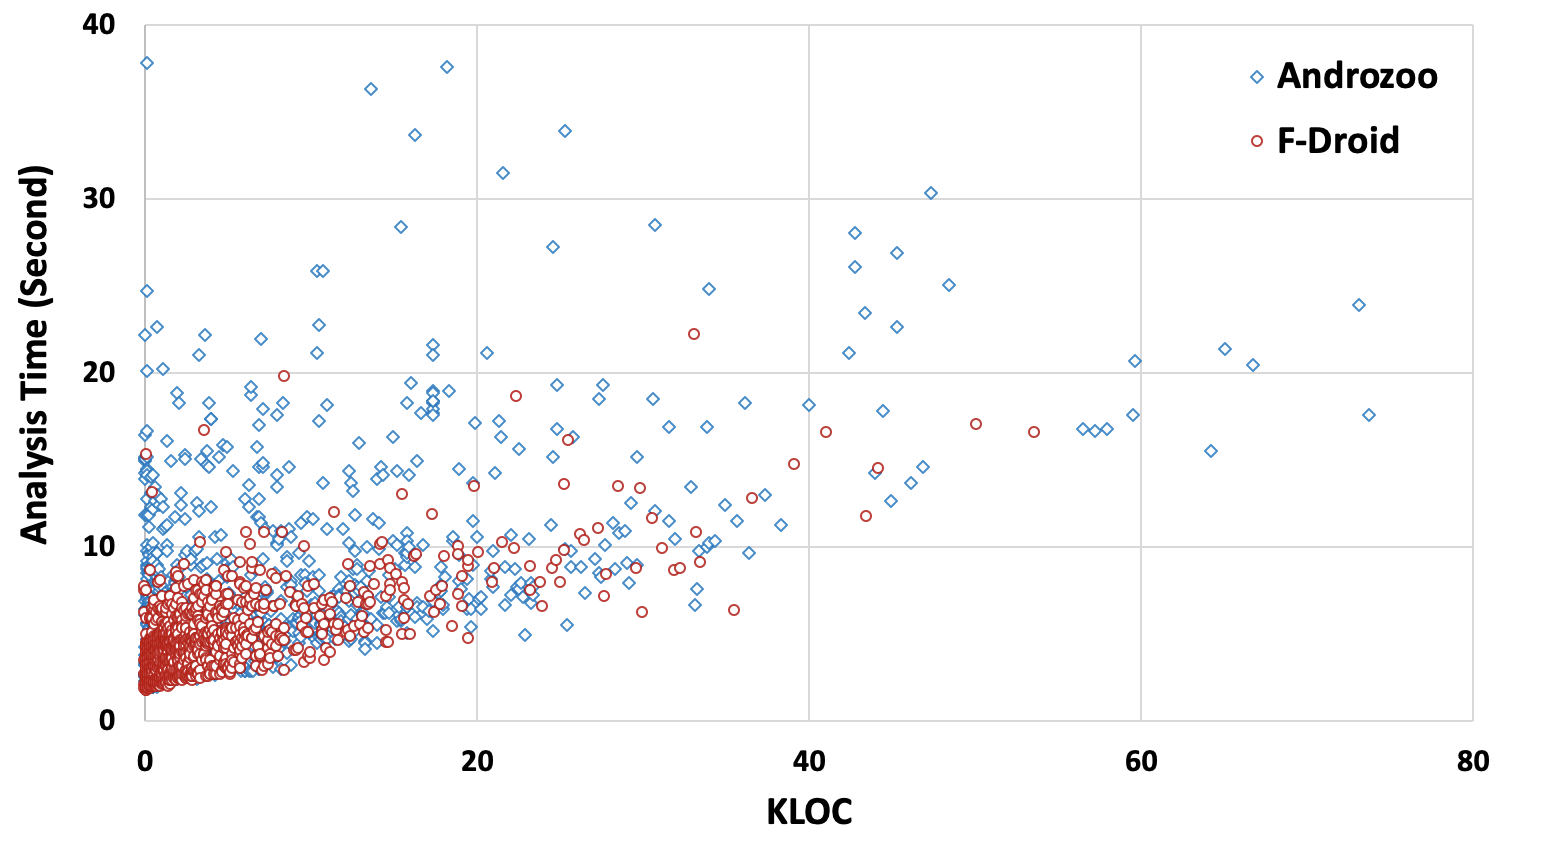
\includegraphics[width=0.46\textwidth]{images/scatterplot.png}
    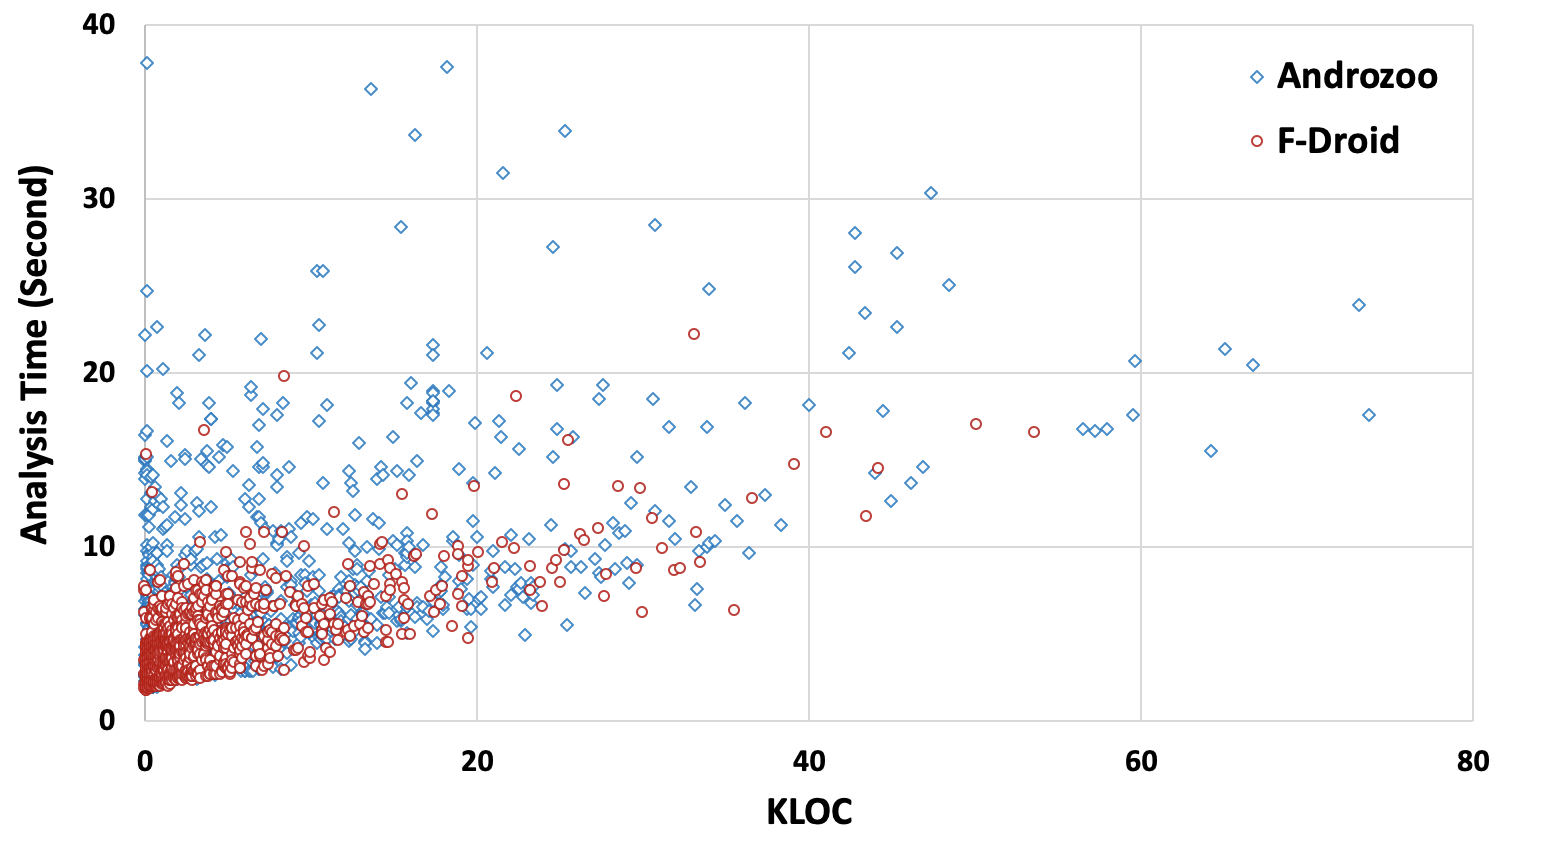
\includegraphics[width=\linewidth]{images/scatterplot.png}
%    \vspace{-0.2cm}
    \caption{Scatter plot representing analysis time for compatibility checking of Android apps using \@approach.}
    \label{fig:scatterplot}
%    \vspace{-0.7cm}
\end{figure}


%\vspace{-7pt}
\subsection{RQ3: Performance} % and Timing}

Table~\ref{tab:tab-timing-results} shows the analysis times
of \@approach, {\sc CiD}, and {\sc Lint} (in seconds).
Dashes indicate that either the corresponding technique fails to produce analysis
results after 600 seconds or crashes.
%timeouts.  after 10 minutes of analysis.
As shown, the analysis time taken by \@approach is
significantly lower than those of \textsc{CiD} and
\textsc{Lint} for almost all the apps. Also note that
\textsc{CiD} fails to completely analyze four apps. %after 600 seconds have passed. 
The average analysis time taken by
\@approach, {\sc CiD}, and {\sc Lint} per app is 5.7, 22.9
and 17.1 seconds respectively, corroborating that \@approach
can efficiently vet Android apps for compatibility issues in
a fraction of time taken by the other state-of-the-art
tools.




Figure~\ref{fig:scatterplot} presents the time taken by \@approach 
to perform compatibility analysis on real-world apps.
The scatter plot depicts both the analysis time and the app size.  
The experimental results show that the average 
analysis time taken by \@approach, {\sc CiD}, and {\sc Lint} per app on
real-world data sets is 6.2 seconds (ranging from 1.6
to 37.8 seconds), 29.5 seconds (ranging from 4.1 to
78.4 seconds), and 24.7 seconds (ranging from 4.7 to
75.6 seconds), respectively. We have found outliers during the analysis. For example, the app in the top left corner in Figure~\ref{fig:scatterplot} is a game application which extensively uses third party libraries, which took a considerable amount of time for the analyzer to compute the data structures required for the compatibility analysis, despite its small KLOC. On the other hand, the app in the right side of the diagram, closer to 80 KLOC, loads three times less library classes than the aforementioned app, implicating in less complex graphs to analyze.  
Overall, the timing results show that \@approach  is up to 8.3 times (4.7 times on average) faster than the state-of-the art techniques, and is able to complete analysis of real-world apps in just a few seconds (on an ordinary laptop), confirming that the presented technology is indeed feasible in practice for real-world usage.



\begin{comment}
\begin{figure}[b!]
	\centering
	\vspace{-0.5cm}
	%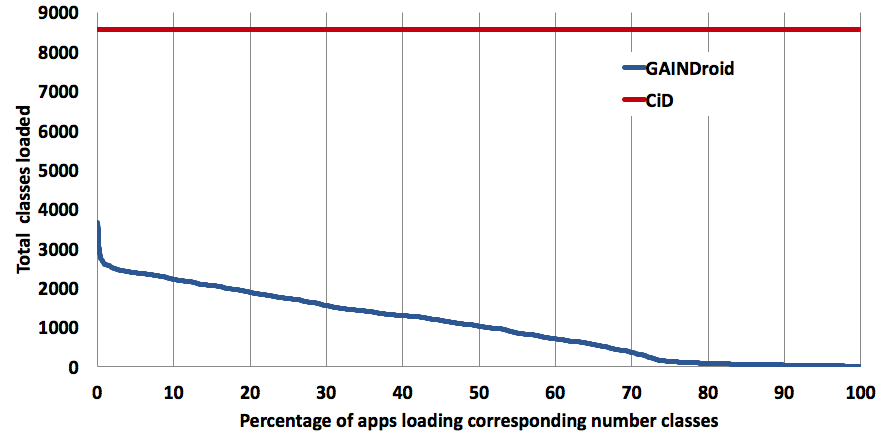
\includegraphics[width=0.48\textwidth]{images/classes.png}
	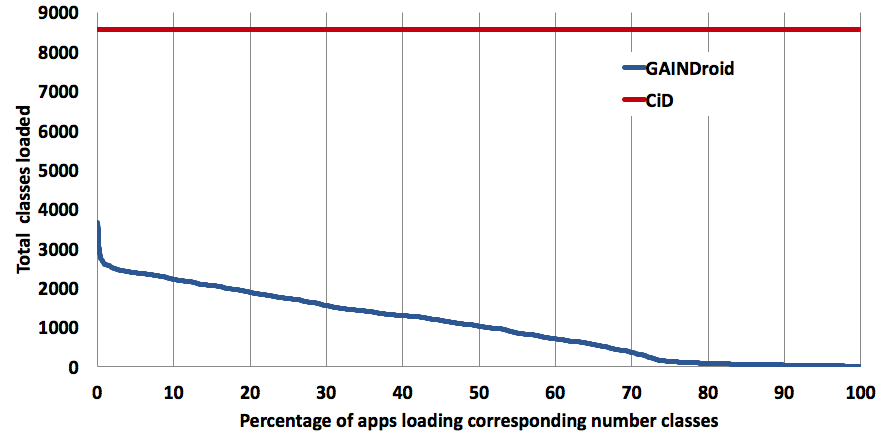
\includegraphics[width=0.9\linewidth]{images/classes.png}
	\vspace{-0.2cm}
	\caption{Number of classes loaded by \@approach and {\sc CiD} when analyzing real-world Android apps.}
	\label{fig:classes_loaded}
	%\vspace{-0.8cm}
\end{figure}
\end{comment}


\begin{figure}[b!]
	\centering
	%    \vspace{-0.8cm}
%	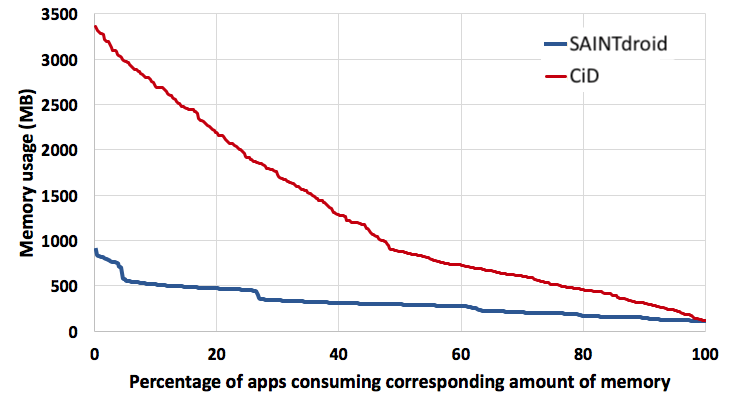
\includegraphics[width=0.42\textwidth]{images/memory_gd.png}
	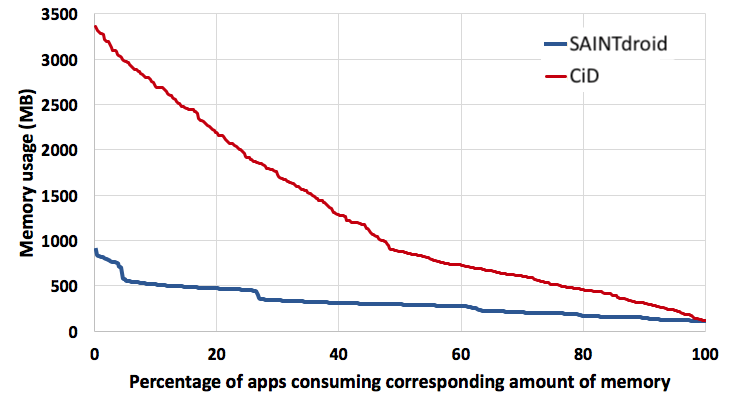
\includegraphics[width=\linewidth]{images/memory_gd.png}
%	\vspace{-0.2cm}
	\caption{Amount of memory used by \@approach and \textsc{CiD} when analyzing real-world Android apps.}
	\label{fig:memory_gd}
%	\vspace{-0.6cm}
\end{figure}

To better understand why \@approach performs more efficient than the state-of-the-art approaches, we conducted further performance evaluation, comparing the amount of
resources and analysis efforts required by each approach. 
\begin{comment}
%Our approach extends a class-loader based program analysis framework while {\sc CiD} is based on {\sc Soot}, which is a compiler based program analysis framework. \textcolor{blue}{To start the performance comparison, we monitored the number of analyzed classes in each approach.}
Since our approach extends a class-loader based program analysis framework rather than a compiler based program analyzer, %---e.g., {\sc CiD} is based on the {\sc Soot} framework---
we expect the efficiency gains in \@approach is due to the effective loading of classes during the analysis. In this set of experiments, we attempted to corroborate our intuition and obtain empirical evidence of this relationship.




We first monitored the number of analyzed classes in each approach.
%We notice that {\sc CiD} needs to load all of the Android classes prior to performing its analysis. On the contrary, \@approach only loads the classes that the app actually uses. 
Figure~\ref{fig:classes_loaded} depicts the number of classes loaded by \@approach and \textsc{CiD} when analyzing real-world apps.
The red line in Figure~\ref{fig:classes_loaded} shows that {\sc CiD} loads all Android classes from the latest available Android framework ~\cite{AndroidAOSP}. 
As of January 2019, there are 8552 classes in the Android framework. 
On the contrary, \@approach only loads the classes that the app actually uses. 
According to the diagram, \@approach, shown by the blue line in Figure~\ref{fig:classes_loaded}, at most loads 3,600 classes, and that only occurs for a very small number of apps. 
Indeed, for over 60\% of the analyzed apps, \@approach loads less than 1,000 classes , which is eight times more efficient compared to \textsc{CiD}. 
%For around 20\% of all real-world apps, \@approach loads just above 2,000 classes (shown by the blue line in Figure~\ref{fig:classes_loaded}). It is also interesting to note that for analyzing 60\% of the apps, \@approach loads less than 1,000 classes, which is 8 times more efficient compared to \textsc{CiD}.

 
%Loading fewer classes also allows \@approach to require less memory to perform its analysis. To investigate this matter, we also monitored the memory footprint required by each approach for performing analysis. Figure~\ref{fig:memory} shows a comparison of how much memory \@approach, {\sc CiD} and {\sc Lint} are using during the analysis of benchmark apps. According to the results, \@approach on average requires 265 MB of memory to perform compatibility analysis, which is by and large similar to what {\sc Lint} requires. {\sc CiD}, on the other hand, needs 1.3 GB (or five times more memory) to perform the same analysis. We have also observed \@approach's memory usage behavior while analyzing a set of real-world apps. As shown in Figure~\ref{fig:memory_gd}, \@approach on average  requires 329 MB (ranging from 898MB to 110MB) to analyze real-world Android apps, corroborating  the effectiveness of the our technique based on a class-loader based approach for compatibility analysis.

Loading fewer classes also allows \@approach to require less memory to perform its analysis. To investigate this matter, we also 
\end{comment}
Specifically, we
monitored the memory footprint required by each approach for performing analysis. Figure~\ref{fig:memory_gd} shows a comparison of how much memory \@approach and {\sc CiD} are using during the analysis of real-world apps. According to the results, \@approach on average requires 329 MB (ranging from 119MB to 898MB) of memory to perform the compatibility analysis. On the other hand, {\sc CiD} on average uses 1.3 GB (or four times more memory) to perform the same analysis. We interpret this data as corroborating  the effectiveness of our technique in practice  %based on a class-loader based approach 
for compatibility analysis.
